\chapter{Le Magnétisme Moléculaire}

Définir précisément ce qu'est un aimant moléculaire n'est pas chose aisé. Il faut bien s\^ur qu'il possède un moment magnétique non nul. Ce moment magnétique peut \^etre de spin, orbital ou bien les deux. Mais cela n'est pas suffisant. Il faut de plus, que ce moment magnétique est une orientation préférentielle. Cela se traduit par l'existence d'un axe facile, c'est à dire deux orientations qui correspondent à un minimum d'énergie pour le moment magnétique. Ces deux conditions sont les conditions minimales à remplir pour parler d'aimant moléculaire. Mais pour mettre en évidence ces propriétés, il faut qu'il soit possible de les mesurer. Autrement dit, l'anisotropie doit \^etre suffisamment forte pour que l'énergie thermique ne puisse pas retourner l'aimantation.

Cependant, l'aimant moléculaire que l'on vient de décrire n'est pas vraiment "sexy" pour reprendre les termes de Wolfgang Wernsdorfer. Ce que l'on souhaite aussi, c'est de pouvoir mettre en évidence des phénomènes quantiques tel que le retournement de l'aimantation par effet tunnel ou Quantum Tunneling of the Magnetization~(QTM) que nous décrirons plus bas. Ceci n'est possible que s'il existe, en plus de l'axe facile, un plan difficile qui permet, comme nous le verrons dans la suite, de coupler les différents états magnétique de la molécule entres eux. De plus, le spin électronique n'est pas toujours l'unique acteur du magnétisme moléculaire. Il arrive parfois que le spin nucléaire joue un r\^ole majeur dans les phénomènes quantique mesurés.

Afin de comprendre la physique associé aux aimants moléculaires, on peut donc procéder par étape. On peut tout d'abord décrire l'origine du moment magnétique non nul d'une molécule. On peut ensuite introduire la notion d'axe facile et comment elle se traduit dans le formalisme quantique. On peut ensuite aborder la notions de plan difficile, son origine et ces conséquences. Enfin, une description des interaction entre spin électronique et spin nucléaire est nécessaire pour décrire de la façon la plus complète certains aimants moléculaire, à base de lanthanide notamment.

\section{L'origine du moment magnétique}
Nous l'avons déjà dit, pour qu'une molécule puisse \^etre appelé aimant moléculaire, il faut tout d'abord qu'elle possède un moment magnétique non nul. Pour arriver à ce résulat, on peut adopter deux stratégies. La première consiste à synthétiser une molécule composé de plusieurs atomes magnétique qui vont interagir entre eux, par l'intermédiaire des ligands, pour donner un moment magnétique résultant non nul. La deuxième technique consiste à n'utiliser qu'un métal magnétique que l'on va venir entourer de ligands non magnétiques.

\subsection{La solution a plusieurs centres}
Cette solution a été la première adopté dans le domaine du magnétisme moléculaire. Elle a permis notamment de synthétiser la désormais célèbre molécule de Mn$_{12}$-ac~(cf Fig.\ref{Mn12}). Cette dernière est composé par douze atomes de Manganèse et autant d'atomes d'oxygène~(qui consituent le coeur magnétique) ainsi que des ligands organiques. Les huit atomes de manganèse en périphérie, de part leur interaction, sont parallèles les uns au autres. Chacun d'eux possédant un spin $S=2$, on se retrouve avec un spin total $S=16$ pour ce qui est de ces huit atomes. Les trois atomes situés au centre du coeur magnétique sont également alignés entre eux pour un spin total de $S=6$~(pour chaque manganèse $S=3/2$). Ces deux groupes étant antiparallèle l'un par raport à l'autre, on obtient un spin total de $S=10$. On comprend ici que le spin total de la molécule n'est pas la simple résultante de l'ensemble des spins qui là compose mais plut\^ot du jeu d'interactions complexe dont elle est le siège. Dans ce cadre, les atomes d'oxygène jouent un r\^ole majeur dans l'interaction dite de "super échange" qui lie les différents atomes de manganèses entre eux. Nous verrons dans la suite lorsque nous aborderons le champ de ligand que l'ensemble de la structure joue en fait un r\^ole dans les propriétés magnétique de la molécule. Cependant, les interactions au sein du coeur magnétique sont celles qui vont déterminer les valeur totale du moment magnétique de l'aimant moléculaire.
\begin{figure}
\centering 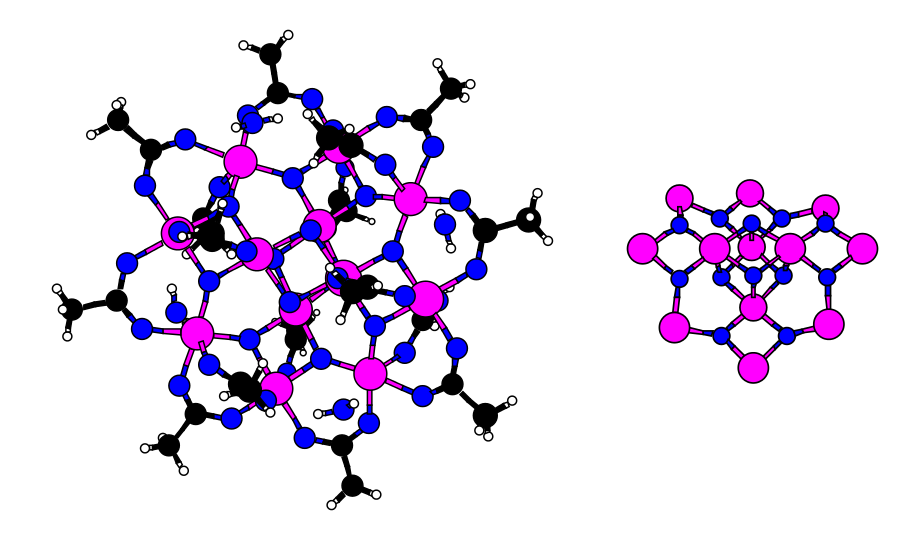
\includegraphics[scale=0.3]{Theorie/MagMol/figure1/Mn12.png} 
\caption{Sur la gauche, la molécule de Mn$_{12}$-ac. Sur la droite, le centre magnétique Mn$_{12}$O$_{12}$. Les quatre manganèses internes de spin $S=3/2$ sont antiparallèles aux huit maganèses de spin $S=2$ situés en périphérie. Le moment magnétique total résultant est $S=10$~(extrait de When Magnetism Goes Nano). Le couplage entre les différents spins est médié par les atomes d'oxygène en bleus sur la figure.}
\label{Mn12}
\end{figure}

\subsection{La solution de l'ion métallique unique}
Dans ce deuxième type d'aimants moléculaires, le moment magnétique total ne dépend que de celui de l'ion qui la compose. Cet ion va \^etre ensuite inséré dans un ligand pour former un aimant moléculaire. Contrairement à ce qui a été présenté précédemment, le moment magnétique total ne dépend donc pas des interactions entre différents centre magnétique. On peut dors et déjà y voir un signe de robustesse, ce type d'ailmant moléculaire étant par construction moins sensible à une déformation de sa structure~(cf chapitre précédent avec l'effet Jhan-Teller). La contre-partie est que par construction, le moment magnétique total est limité à celui de l'ion composant l'aimant moléculaire alors que dans le premier cas, une construction habile peut donner des moment magnétique de l'ordre de plusieurs dizaine de $\mu_b$. Un dex exemple les plus étudier est celui du "double-decker"~(nommé en référence aux avions à deux ailes) où plusieurs ion peuvent \^etre choisi comme centre magnétique. Dans notre cas, nous utiliserons le TbPc$_2$ où terbium "double-decker".

\begin{figure}
\centering 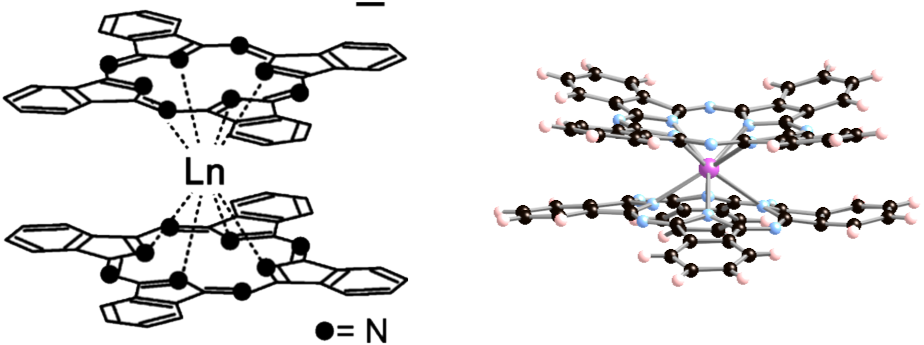
\includegraphics[scale=0.5]{Theorie/MagMol/figure2/figure2.png} 
\caption{A gauche, structure générale d'un "double decker" à base de Lanthanide~(noté Ln - tiré de Ishikawa, Single molecule magnet with single lanthanide ion). A droite, vu d'artiste de cette m\^eme molécule. Les atomes d'azote sont représentés en bleu, ceux de carbone en noir, ceux hydrogènes en beige et l'atome lanthanide en mauve}
\label{TbPc2}
\end{figure}

\section{Hamiltonien d'un aimant moléculaire "standard"}
\subsection{L'axe facile}
Comme nous le disions plus haut, le ligand a aussi une influence sur le magnétisme de la molécule. Cette influence peut \^etre prise en compte par l'introduction d'un champ de ligand. L'origine de ce champ de ligand est purement Coulombienne
 et dépend très fortement des symétrie du système. On utilise pour rendre compte de ce phénomène les opérateurs de Stevens rappelé en annexe. Pour notre introduction, nous allons nous concentrer sur le terme le plus simple qui peut introduire un axe facile à savoir:
 \begin{eqnarray}
E_{ani} = -DS_z^2 \nonumber
\end{eqnarray}
où $D$ est le paramètre d'anisotropie, $S_z$ la composante en $z$ du moment magnétique et $E_{ani}$ la modification de l'énergie du système du à cette anisotropie. Si $D>0$, nous avons à faire à un axe difficile et le moment magnétique se trouvera de préférence dans le plan perpendiculaire à l'axe $z$. Si $D<0$, nous avons un axe facile et le moment magnétique sera aligné le long de l'axe z.

\subsection{L'effet Zeeman}
Comme tout système magnétique, un aimant moléculaire est sensible au champ magnétique. Celui si va venir faire varier l'énergie du système de la valeur
\begin{eqnarray}
E_{Zeeman}= g\mu_b \mathbf{BS} \nonumber
\end{eqnarray}
ou $E_{Zeeman}$ est l'énergie associé à l'effet Zeeman, $g$ le facteur de Landé, $\mu_b$ le magnéton de Bohr, $B$ le champ magnétique appliqué et $S$ le moment magnétique du système. Si maintenant ce champ magnétique est appliqué celon l'axe $z$ du système, cette expression devient :
\begin{eqnarray}
E_{Zeeman}= g\mu_b B S_z \nonumber
\end{eqnarray}

\subsection{Le plan difficile}
De m\^eme que nous pouvons avoir un axe facile( ou difficile), on peut égalment rencontrer un plan difficile(~ou facile). Encore une fois, celui-ci est directement induit par le champ de ligand et donc dépend des symétries du système. Il peut \^etre exprimé deux façons rigoureusement équivalente :
\begin{eqnarray}
E_{plan} = E ( S_x^2 -S_y^2) \nonumber
\end{eqnarray}
ou bien encore
\begin{eqnarray}
E_{plan} = \frac{E}{2} ( S_+^2  + S_-^2) \nonumber \\
\end{eqnarray}
où $S_x$ et $S_y$ sont les projection du moment magnétique dans le plan $(x,y)$, $S_+$ et $S_-$ les opérateurs création anhilation, $E$ est le paramètre d'anysotropie et $E_{plan}$ l'énergie associé à la présence d'un plan difficile. La présence des termes création anhilation n'est pas sans conséquence sur le système. En effet, ce terme va venir coupler les différentes valeur $m_z$. On verra plus tard quelles sont les conséquences d'un tel couplage. On peut cependant déjà remarqué que la base $(S,S_z)$ n'est plus une bonne base pour décrire le système.

\subsection{L'effet Zeeman}
Comme tout système magnétique, un aimant moléculaire est sensible au champ magnétique. Celui si va venir faire varier l'énergie du système de la valeur
\begin{eqnarray}
E_{Zeeman}= g\mu_b \mathbf{BS} \nonumber
\end{eqnarray}
ou $E_{Zeeman}$ est l'énergie associé à l'effet Zeeman, $g$ le facteur de Landé, $\mu_b$ le magnéton de Bohr, $B$ le champ magnétique appliqué et $S$ le moment magnétique du système. Si maintenant ce champ magnétique est appliqué celon l'axe $z$ du système, cette expression devient :
\begin{eqnarray}
E_{Zeeman}= g\mu_b B S_z \nonumber
\end{eqnarray}

\subsection{La cas du Fe$_8$}
Si l'on synthétise ce qui vient d'\^etre présenté, un aimant moléculaire soumit à un champ magnétique $B$ appliqué suivant l'axe $z$ possède l'hamiltonien suivant:
\begin{eqnarray}
E =  -DS_z^2 + \frac{E}{2} ( S_+^2  + S_-^2) + g\mu_b B S_z 
\end{eqnarray}


Nous allons maintenant appliqué cet hamiltonien à l'étude d'un aimant très utiliser dans les expériences relativer au magnétisme moléculaire : le Fe$_8$. Nous avons déjà vu l'influence de l'effet Zeeman et de l'axe facile sur les spectre en énergie d'un système. Ici, nous allons nous intéresser plus particulièrement à la présence d'un plan difficile est voir comment se plan vient perturber le système. Nous avons donc tracer le diagramme Zeeman de la molécule de Fe$_8$ en ne tenant pas compte de la présence d'un plan facile et ensuite en l'introduisant dans l'hamiltonien du système. On constante tout d'abord une altération forte de l'allure générale du diagramme Zeeman. Mais plus important que cela, nous voyons apparaitre des zones où, au lieu de se croise, les niveaux d'énergie ont l'air de "s'éviter" : on parle d'anti-croisement. La présence de ces anti-croisements témoigne du couplage entre les différents état de l'aimantation du système. Nous allons à present étudier les conséquence d'un tel couplage. Pour cela, nous utiliserons la cas simple d'un spin $1/2$ soumis à un champ magnétique.